% !TEX root = ../Coherence.tex

\section{Introduction} 
\label{s:introduction}


\begin{enumerate}

    \item Polytopal coherence theorem -- Section 2

    \item Categorified ns operad + application of the theorem, proof of isomorphism with K. Do{\v s}en and Z. Petri{\'c} in \cite{DP15} -- Section 3

    \item Rewriting -- Section 4
    
    \item General Koszulity theorem -- Section 5

    \item Link with Poincar\'e duality and open questions -- Section 6

\end{enumerate}


%%%%%%%%%%%%%%%%%%%%%%%%%%%%%%%%


\subsection{Coherence and rewriting for monoidal categories}

We start from a set $X$, considered as a set of  ``object variables"  (they are meant to be interpreted as objects in some category).  We define two sets   of object terms and morphism terms, respectively:
$$\begin{array}{l}
T::= x\  \;(\mbox{where}\;x\in X) \Alt I \Alt T\otimes T\\
M ::= \alpha \Alt \lambda \Alt\rho\Alt  \alpha^{-1} \Alt \lambda^{-1} \Alt\rho^{-1} \Alt M\comp M\Alt \id\Alt M\otimes M
\end{array}$$
In English, an object term is either a variable $x$, or $I$, or, if $s,t$ are object terms, then so is $(s\otimes t)$.
We actually only consider {\em well-typed} morphism terms  which are the ones accepted by the following typing rules, involving judgements of the form $M:T_1\rightarrow T_2$:
$$\seq{}{\alpha:(T_1\otimes T_2)\otimes T_3\rightarrow T_1\otimes(T_2\otimes T_3)}\quad\quad
\seq{}{\lambda:I\otimes T\rightarrow T}\quad\quad\seq{}{\rho:T\otimes I\rightarrow T}$$
$$\seq{}{\alpha^{-1}:T_1\otimes(T_2\otimes T_3)\rightarrow (T_1\otimes T_2)\otimes T_3}\quad\quad
\seq{}{\lambda^{-1}: T\rightarrow I\otimes T}\quad\quad\seq{}{\rho^{-1}:T\rightarrow T\otimes I}$$

$$\seq{}{\id:T\rightarrow T}\quad\quad \seq{M_1:T_1\rightarrow T_2\quad M_2:T_2\rightarrow T_3}{M_2\comp M_1:T_1\rightarrow T_3}\quad\quad \seq{M_1:T_1\rightarrow T'_1\quad M_2:T_2\rightarrow T'_2}{M_1\otimes M_2:T_1\otimes T_2\rightarrow T'_1\otimes T'_2}$$
In English, the formal typing rules read as: if all the typing assertions above the horizontal bar hold, then the typîng assertion below the bar holds.

One quotients the set of morphism terms by the laws of categories and of bifunctors, and by Mac Lane's coherence equations.
What one then obtains is the free monoidal category ${Free}(X)$ over $X$ i.e., for every {\em function} $\rho:X\rightarrow \cat{C}$ (mapping each $x$ to an object of  a monoidal category $\cat{C}$) there exists a unique strict monoidal functor $\dl \_\dr^\rho_{\cat{C}}:{Free}(X)\rightarrow\cat{C}$ that extends it.

The coherence theorem asserts that for any two terms $M,M':T\rightarrow T'$  of the {\em same type} we have $\dl M\dr^\rho_{\cat{C}}=\dl M'\dr^\rho_{\cat{C}}$  (for any monoidal category, and any valuation).


%%%%%%%%%%%%%%%%%%%%%%%%%%%%%%%%%%%%%%%%

\subsection{Reminders on hypergraph polytopes}

A hypergraph is given by a set  $H$ of vertices (the carrier), and a subset 
$\hyper{H}\inc {\mathcal{P}}(H)\backslash\emptyset$ such that $\Union \hyper{H}=H$.
 The elements of $\hyper{H}$ are called the {\em hyperedges} of $\hyper{H}$.  
 We always assume that $\hyper{H}$ is {\em atomic}, by which we mean that 
 $\set{x}\in \hyper{H}$, for all $x\in H$. 
 Identifying $x$ with $\set{x}$, $H$ can be seen as the set of  hyperedges of 
 cardinality $1$, also called {\em vertices}. We shall use the convention to 
 give the same name to the hypergraph and to its carrier, in different fonts. 
 %When this convention cannot be used, we use the notation $V(\hyper{H})$ for the set of vertices of $\hyper{H}$.
% In the sequel, we shall write $\hyper{H}$ for an atomic  hypergraph, and $H$ for its set of vertices, i.e. 
%$H=\Union\hyper{H}$.
A hyperedge of cardinality 2 is called an {\em edge}.  Note that any ordinary graph $(V,E)$ can be viewed as the atomic hypergraph
$\setc{\set{v}}{v\in V} \union \setc{e}{e\in E}$ (with no hyperedges of cardinality $\geq 3$). 

\smallskip
 
If $\hyper{H}$ is a hypergraph,  and if  $X\inc H$, we set
$\hyper{H}_X:=\setc{Z}{Z\in \hyper{H}\;\mbox{and}\; Z\inc X}$, and $\restrH{H}{X}=\hyper{H}_{H\backslash X}$.
We say that $\hyper{H}$ is {\em connected} if there is no non-trivial partition $H=X_1\union X_2$ such that $\hyper{H}=\hyper{H}_{X_1}\union \hyper{H}_{X_2}$, and that $X\inc H$ is connected in $\hyper{H}$ if $\hyper{H}_X$ is connected.
%All our hypergraphs will be finite. 
For each finite hypergraph there exists a partition
$H=X_1\union\ldots\union X_m$ such that each $\hyper{H}_{X_i}$ is connected and $\hyper{H}=\Union(\hyper{H}_{X_i})$.  The $\hyper{H}_{X_i}$'s are  the {\em connected components} of $\hyper{H}$. The notation
$\hyper{H},X  \leadsto \hyper{H}_1,\ldots, \hyper{H}_n$
 will mean that  $\hyper{H}_1,\ldots,\hyper{H}_n$ are  the
 connected components of $\restrH{H}{X}$.  
%We shall  write
%$\hyper{H}_i$  for
%$\hyper{H}_{H_i}$. 

\smallskip

Do\v sen and Petri\'c~\cite{DP} have proposed the following insightful reading of the data of a finite connected hypergraph $\hyper{H}$ as a truncated simplex: the elements of $H$ are identified with the facets (i.e. codimension 1 faces) of the $(|H|-1)$-dimensional simplex, and each $\emptyset\incs X\incs H$, $|X|\geq 2$, such that    $\hyper{H}_X$ is connected designates the intersection of the facets in $X$ as a face to be truncated.
The obtained polytopes, called \emph{hypergraph polytopes}, extend the construction of graph associahedra \cite{CD-CCGA, Zel06}, and are equivalent to nestohedra, as introduced by Postnikov \cite{P09}.  Moreover,  the faces of the   polytope obtained by performing  all the prescribed truncations  are labeled by non-planar trees whose nodes are decorated by non-empty subsets of $H$, called {\em constructs}, whose recursive definition  we give next using a syntax introduced in \cite{COI}:

\smallskip
Let  $\emptyset\neq Y\subseteq H$. If   $\hyper{H},Y  \leadsto \hyper{H}_1,\ldots, \hyper{H}_n$, and if  $T_1,\ldots,T_n$ are constructs of $\hyper{H}_1,\ldots,\hyper{H}_n$, respectively, then the tree obtained by grafting $T_1,\ldots,T_n$ on the root node decorated by $Y$, denoted by $Y(T_1,\ldots,T_n)$, is a construct of  $\hyper{H}$~\footnote{\label{construct-tubing} Constructs are in one-to-one correspondence with tubings as defined in \cite{CD-CCGA}: for a given construct $T$, each tube of the associated tubing is given by a node of $T$ and all its descendance. There are  as many tubes in the tubing as nodes in the construct.}. We write $Y=\mbox{root}(Y(T_1,\ldots,T_n))$.

\smallskip
 The base case is when $Y=H$ (and hence $n=0$): then the one-node tree $H()$ (written simply $H$) is a construct.
We write $T:\hyper{H}$ to denote that $T$ is a construct of $\hyper{H}$. 
The formalism of constructs   allows us to view the inclusion of faces of a hypergraph polytope through the process of contracting tree edges: by contracting an edge of a construct and  merging the decorations of the two nodes related by that edge, one gets a covering construct.

\smallskip
Simplices are ``encoded'' as the hypergraphs  $$\hyper{S}^X=\setc{\set{x}}{x\in X}\union\set{\set{X}}$$ (no truncation prescribed). The constructs have the form $Y(\ldots,\set{y},\ldots)$ where $\emptyset\incs Y\inc X$ and $y$ ranges over $H\backslash Y$, and are therefore isomorphic to multipointed sets. In order to illustrate  how the hypergraph structure dictates truncations, consider the hypergraph $\hyper{H}=\set{\set{x},\set{y},\set{z},\set{y,z}, \set{x,y,z}}$, obtained from $\hyper{S}^{\{x,y,z\}}$ by adding the edge $\{y,z\}$. The construct 
 $\set{x}(\set{y},\set{z}):\hyper{S}^{\{x,y,z\}}$ is {\em not} a construct of $\hyper{H}$, since $\hyper{H}_{\set{y,z}}$ is connected.  Instead, $\hyper{H}$ features 3 new constructs: 
$\set{x}(\set{y}(\set{z}))$, $\set{x}(\set{z}(\set{y}))$ and $\set{x}(\set{y,z})$, encoding two  vertices and one edge, obtained by truncating  the vertex $\set{x}(\set{y},\set{z})$ of $\hyper{S}^{\{x,y,z\}}$.

As a slightly more involved example, we show in Figure \ref{hemiassoc} the polytope encoded by the hypergraph $\hyper{H}=\{\{x\},\{y\},\{u\},\{v\},\{x,y\},\{x,u\},\{x,v\},\{u,v\},\{x,u,v\}\}$, obtained from the  tetrahedron by truncating three of its vertices and four of its edges. We also ``zoom in'' into the square obtained by the truncation prescribed by $\{u,v\}$  and label its four 1-dimensional and four 0-dimensional faces by the appropriate constructs of $\hyper{H}$. 

% !TEX root = ../Coherence.tex

\begin{figure}
\centering
  \resizebox{4cm}{!}{
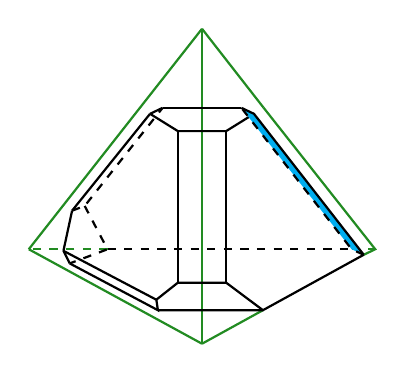
\begin{tikzpicture}[thick,scale=2]
\coordinate (A1) at (0,2);
\coordinate (A11) at (-0.39,1.5);
\coordinate (A111) at (-0.25,1.498);
\coordinate (A112) at (-0.33,1.46);
\coordinate (A12) at (0.39,1.5);
\coordinate (A121) at (0.25,1.498);
\coordinate (A122) at (0.33,1.46);
\coordinate (A13) at (0,1.25);
\coordinate (A131) at (-0.153,1.35); 
\coordinate (A132) at (0.153,1.35); 
\coordinate (A2) at (0,0); 
\coordinate (A21) at (-0.387,0.213); 
\coordinate (A211) at (-0.29,0.2795); 
\coordinate (A212) at (-0.28,0.213); 
\coordinate (A22) at (0.387,0.213); 
\coordinate (A23) at (0,0.5); 
\coordinate (A231) at (-0.153,0.388); 
\coordinate (A232) at (0.153,0.388); 
\coordinate (A3) at (-1.1,0.6);
\coordinate (A31) at (-0.9,0.49);
\coordinate (A311) at (-0.88,0.59);
\coordinate (A312) at (-0.84,0.51);
\coordinate (A32) at (-0.8,0.976);
\coordinate (A321) at (-0.825,0.845);
\coordinate (A322) at (-0.745,0.875);
\coordinate (A33) at (-0.6,0.6);
\coordinate (A4) at (1.1,0.6);
\coordinate (A41) at (1.027,0.565);
\coordinate (A42) at (0.95,0.6);
%\draw[draw=none,fill=cyan!40,opacity=0.5] (A42)--(A41)--(A121)--(A122)-- cycle;
\draw[draw=ForestGreen]  (A3)--(A2);
\draw[draw=ForestGreen]  (A1)--(A12);
\draw[draw=ForestGreen] (A2)--(A22);
\draw[draw=ForestGreen] (A2) -- (A1);
\draw[draw=ForestGreen] (A3)--(A1);
\draw[draw=ForestGreen,dashed]  (A33) -- (A3);
\draw[draw=ForestGreen,dashed]  (A42) -- (A4);
\draw[draw=ForestGreen] (A41)--(A4)--(A12);
 \draw[draw=black,fill=none]   (A321)--(A311);
 \draw[draw=black,fill=none] (A212)-- (A22) -- (A41);
\draw (A311)--(A312);
\draw (A111)--(A121);
\draw (A111)--(A112);
\draw (A311)--(A211)--(A212) --(A312);
\draw (A112)--(A321);
\draw[dashed] (A321)--(A322)--(A111);
\draw  (A211)--(A231)--(A232)--(A22);
\draw[dashed]  (A33) -- (A42);
\draw (A231) -- (A131) -- (A132) -- (A232) -- cycle;
\draw[dashed] (A322) -- (A33) -- (A312);
\draw (A112) -- (A131) --(A132)--(A122);
\fill[cyan] (A41) -- (A42) -- (A121)--(A122)--cycle;
\draw[dashed]  (A41) -- (A42) -- (A121); 
\draw (A41)--(A122) --(A121);
\end{tikzpicture}} \quad\quad  
\raisebox{1em}{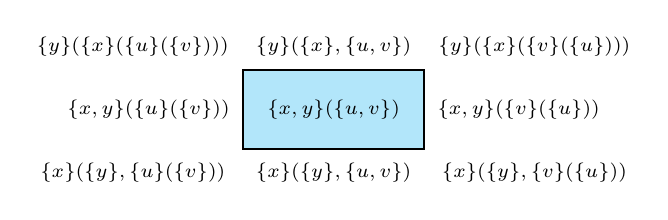
\begin{tikzpicture}[thick]
\coordinate (S1) at (-0.15,0);
\coordinate (S2) at (2.15,0);
\coordinate (S3) at (2.15,1);
\coordinate (S4) at (-0.15,1);
\draw[fill=cyan,opacity=0.3] (S1)--(S2)--(S3)--(S4)-- cycle;
\draw (S1)--(S2)--(S3)--(S4)-- cycle;
\node (s1) at (-1.55,-0.3) {\scriptsize $\{x\}(\{y\},\{u\}(\{v\}))$};
\node (s2) at (3.55,-0.3) {\scriptsize $\{x\}(\{y\},\{v\}(\{u\}))$};
\node (s4) at (-1.55,1.3) {\scriptsize $\{y\}(\{x\}(\{u\}(\{v\})))$};
\node (s3) at (3.55,1.3) {\scriptsize $\{y\}(\{x\}(\{v\}(\{u\})))$};
\node (s14) at (-1.35,0.5) {\scriptsize $\{x,y\}(\{u\}(\{v\}))$};
\node (s23) at (3.35,0.5) {\scriptsize $\{x,y\}(\{v\}(\{u\}))$};
\node (s12) at (1,-0.3) {\scriptsize $\{x\}(\{y\},\{u,v\})$};
\node (s34) at (1,1.3) {\scriptsize $\{y\}(\{x\},\{u,v\})$};
\node (s) at (1,0.5) {\scriptsize $\{x,y\}(\{u,v\})$};

\end{tikzpicture}}
\caption{A truncated simplex. \label{hemiassoc}}
\end{figure}

We recover associahedra and permutohedra as  linear and complete graphs, respectively: 

$$\begin{array}{ll}
\hyper{K}^X= \set{\set{x_1},\ldots,\set{x_n},\set{x_1,x_2},\ldots,\set{x_{n-1},x_n},\set{x_1,\ldots x_n}}, \\
\hyper{P}^X= \set{\set{x_1},\ldots,\set{x_n},\set{x_1,\ldots x_n}} \cup \setc{\set{x_i,x_j}}{1\leq i\neq j\leq n},
\end{array}$$



